%
% $Id: $
%
%
% Compilar a .pdf con LaTeX (pdflatex)
% Es necesario instalar Beamer (paquete latex-beamer en Debian)
%

%
% Gr�ficos:
% Los gr�ficos pueden suministrarse en PNG, JPG, TIF, PDF, MPS
% Los EPS deben convertirse a PDF (usar epstopdf)
%

\documentclass{beamer}
\usetheme{Warsaw}
%\usebackgroundtemplate{
\includegraphics[width=\paperwidth]{format/libresoft-bg.png}}
%\usepackage[spanish]{babel}
\usepackage[latin1]{inputenc}
\usepackage{graphics}
\usepackage{amssymb} % Simbolos matematicos
\usepackage{url}
\usepackage{multirow}


%\definecolor{libresoftgreen}{RGB}{162,190,43}
%\definecolor{libresoftblue}{RGB}{0,98,143}

%\setbeamercolor{titlelike}{bg=libresoftgreen}

%% Metadatos del PDF.
\hypersetup{
  pdftitle={Comparing Computational Thinking Development Assessment Scores with Software Complexity Metrics},
  pdfauthor={Jes�s Moreno-Le�n, Gregorio Robles, Marcos Rom�n-Gonz�lez},
  pdfcreator={KGB-L3 \\ Universidad Rey Juan Carlos},
  pdfproducer=PDFLaTeX,
  pdfsubject={},
}
%%

\begin{document}

\title{Comparing Computational Thinking Development Assessment Scores with Software Complexity Metrics}
\subtitle{}
\institute{jesus.moreno@programamos.es, grex@gsyc.urjc.es, mroman@edu.uned.es \\
KGB-L3, Universidad Rey Juan Carlos}
\author{Jes�s Moreno-Le�n, Gregorio Robles, Marcos Rom�n-Gonz�lez}
\date{IEEE EDUCON 2016, Abu Dhabi, April 11\textsuperscript{th} 2016}

\frame{
\maketitle
\begin{center}

\includegraphics[width=2cm]{format/libresoft-logo}
\hspace{0.5cm}

\includegraphics[width=5cm]{format/gsyc-urjc}
\vspace{0.5cm}

\includegraphics[width=3cm]{format/emadrid.png}
\end{center}
}


% Si el titulo o el autor se quieren acortar para los pies de p�gina
% se pueden redefinir aqu�:
%\title{Titulo corto}
%\author{Autores abreviado}

%% LICENCIA DE REDISTRIBUCION DE LAS TRANSPAS
\frame{
~
\vspace{3cm}

\begin{flushright}

\includegraphics[width=2.2cm]{figs/by-sa}

{\tiny
(cc) 2016 Jes�s Moreno-Le�n, Gregorio Robles and Marcos Rom�n-Gonz�lez\\
  Some rights reserved. This work licensed under Creative Commons \\
  Attribution-ShareAlike License. To view a copy of full license, see \\
  http://creativecommons.org/licenses/by-sa/3.0/ or write to \\
  Creative Commons, 559 Nathan Abbott Way, Stanford, \\
  California 94305, USA. \\
\ \\
Some of the figures have been taken from the Internet \\
Source, and author and licence if known, is specified. \\
For those images, \emph{fair use} applies.
}
\end{flushright}
}
%%

\section{EDUCON 2016, Abu Dhabi}


%--------------------------------------------------------
%\usebackgroundtemplate{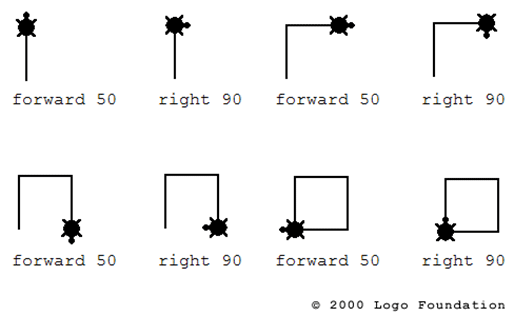
\includegraphics[height=10cm]{figs/turtles.png}}
% background: http://www.wim-network.org/wp-content/uploads/2012/04/iceberg.jpg

\begin{frame}
\frametitle{Code to learn (I)}
\begin{columns}[T]
  \begin{column}{0.5\textwidth}
    \begin{figure}[t!]
      \begin{center}
	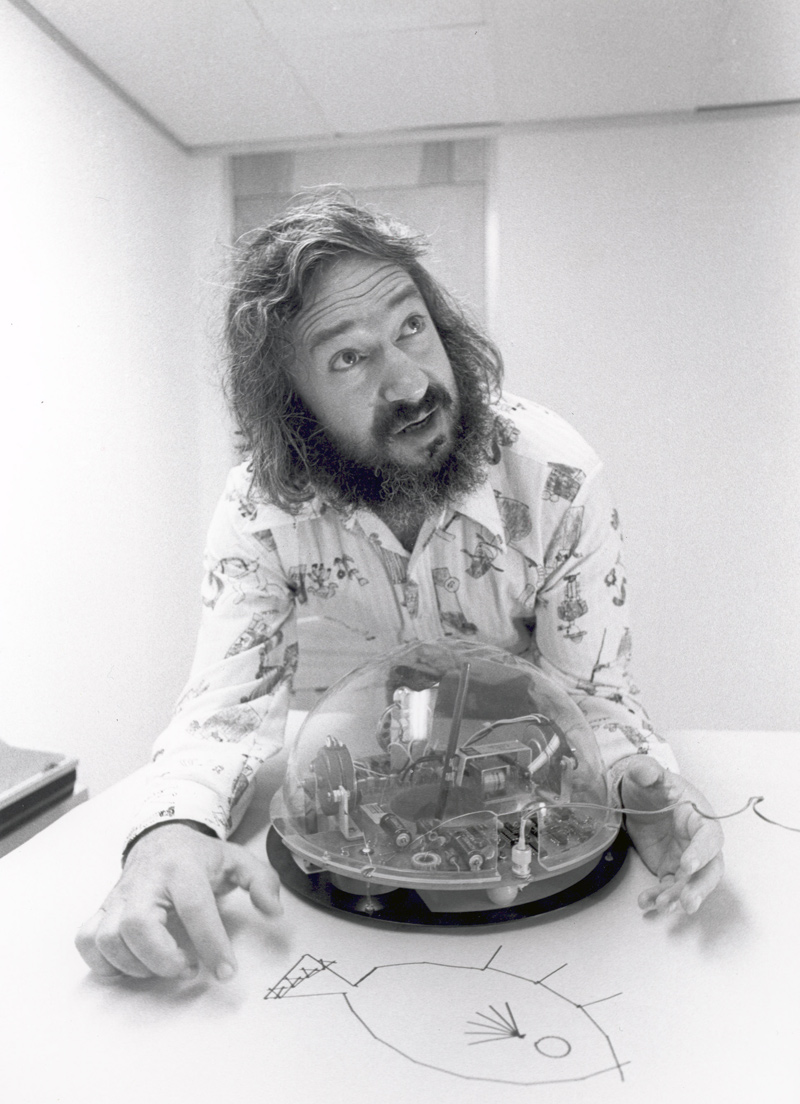
\includegraphics[width=5cm]{figs/seymour.jpg}
      \end{center}
      \label{fig:repetition1}
    \end{figure}
  \end{column}
  \begin{column}{0.5\textwidth}
    \begin{block}{Logo programming language}
      \begin{itemize}
	 \item Developed in the 1960s
         \item Its educational impact was intensively investigated in the 70s and 80s
         \item Students' improvements in maths (and other disciplines) were proved
         \item ``Disappeared'' from the educational landscape since mid-90s
      \end{itemize}
    \end{block}
    \hfill{\Tiny Seymour Papert's picture: jgora.net}
  \end{column}
\end{columns}
\end{frame}

\usebackgroundtemplate{}
%--------------------------------------------------------
\usebackgroundtemplate{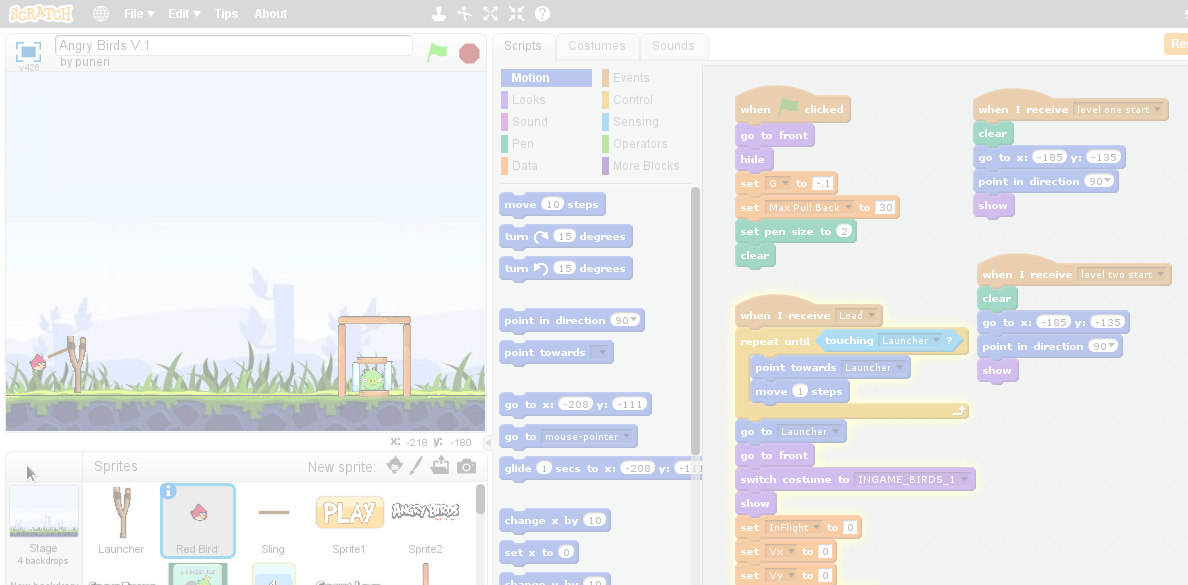
\includegraphics[width=18cm]{figs/AngryBirds2.png}}
\begin{frame}
\frametitle{Code to learn (and II)}

\begin{columns}[T]
  \begin{column}{1\textwidth}
     \begin{block}{Computational Thinking is back in town}
       \begin{itemize}
	 	 \item Alice, Greenfoot, Kodu, \textbf{Scratch}...
         \item Code.org, EU Code Week, Africa Code Week, ArabCode.org...
         \item If there is no evidence showing educational impact of programming, this resurgence of programming in schools could disappear in a few years.
       \end{itemize}
    \end{block}
  \end{column}
\end{columns}

\end{frame}
\usebackgroundtemplate{}

%--------------------------------------------------------
\begin{frame}
\frametitle{Dr. Scratch: Analysis of CT skills}

\begin{figure}[t!]
\begin{center}
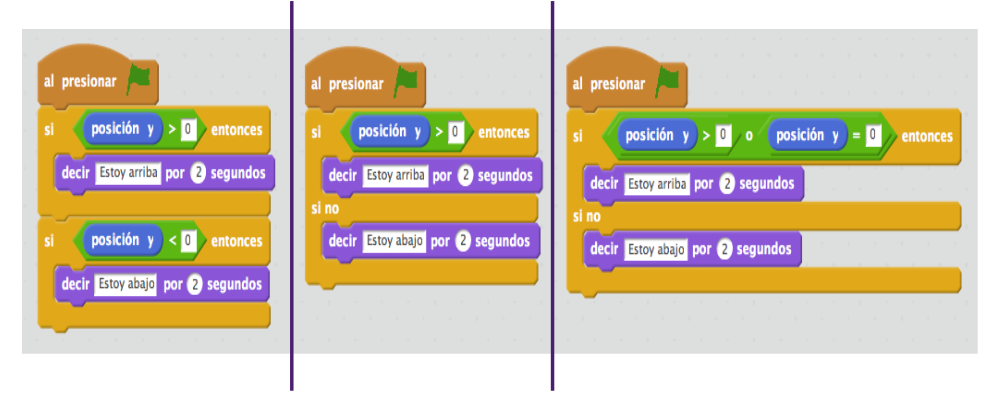
\includegraphics[width=11cm, height=5cm]{figs/logica.png}
\end{center}
\label{fig:logic}
\end{figure}
\begin{center}
Measuring logic development skills
\end{center}
\end{frame}



%--------------------------------------------------------
\begin{frame}
\frametitle{Dr. Scratch: Analysis of CT skills}

\begin{itemize}
  \item Dr. Scratch allows learners to evaluate their projects to receive a computational thinking score
  \item Gamified feedback with tips and tricks
  \item The computational thinking score ranges from 0 to 21 points
  \item It is based on the degree of development of different dimensions of the computational thinking competence:
  \begin{enumerate}
    \item abstraction and problem decomposition
    \item logical thinking
    \item synchronization
    \item parallelism
    \item algorithmic notions of flow control
    \item user interactivity
    \item and data representation
  \end{enumerate}
\end{itemize}
\end{frame}

%--------------------------------------------------------
\begin{frame}
\frametitle{Dr. Scratch: Analysis of CT skills}

\begin{figure}[t!]
\begin{center}
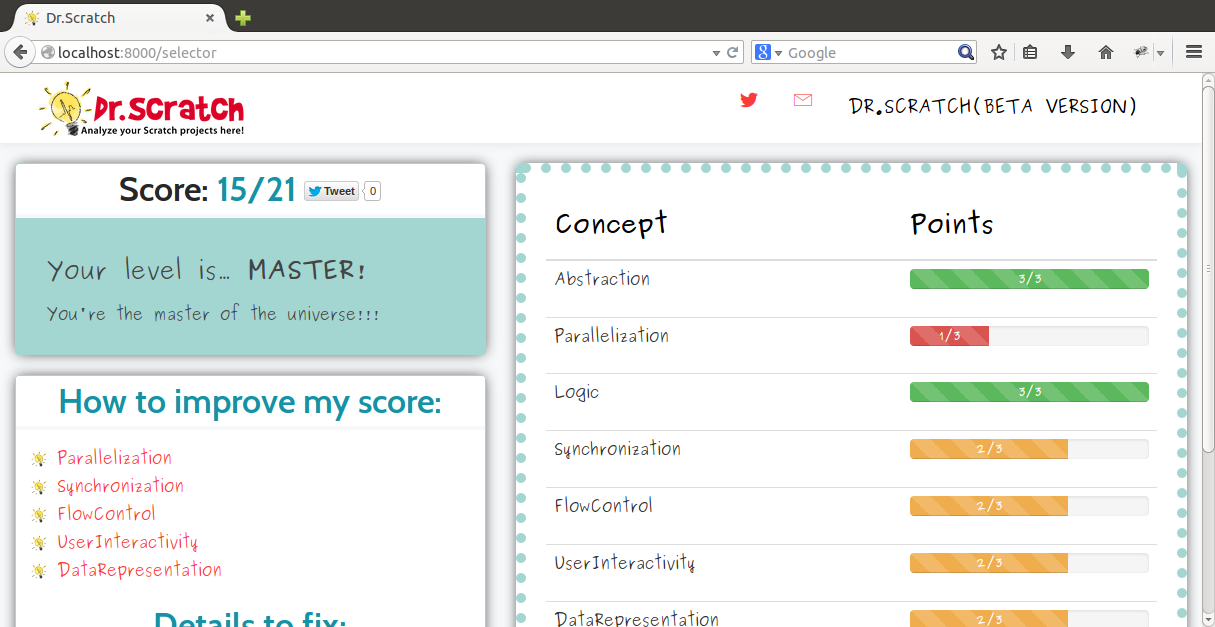
\includegraphics[width=11cm, height=6.1cm]{figs/master.png}
\end{center}
\label{fig:drscratch}
\end{figure}
\begin{center}
Example Dr. Scratch feedback: http://www.drscratch.org
\end{center}
\begin{center}

\end{center}
\end{frame}



%-----------------------    ---------------------------------

%--------------------------------------------------------
\begin{frame}
\frametitle{Classic Software Complexity Metrics}

\begin{itemize}
  \item Cyclomatic Complexity (CC)
  \begin{itemize}
    \item is a graph-theoretic complexity measure that can be used to manage and control program complexity.
    \item based on the number of linear independent paths in a program, and can be used to establish the number of test cases in the basis path testing methodology.
  \end{itemize}
  \item Halstead's metrics
  \begin{itemize}
    \item identifiy certain properties of a program that can be measured and the relationships between them to assess software complexity.
    \item widely used in software engineering to estimate maintenance efforts and guide software testing by identifying complex, hard to maintain modules. 
    \end{itemize}
  \end{itemize}
\end{frame}


%-----------------------    ---------------------------------

\begin{frame}
\frametitle{Example Scratch program}
\begin{center}
	\begin{figure}[t!]
		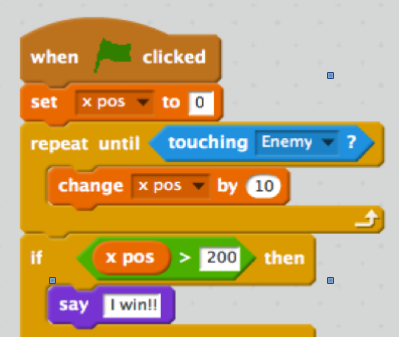
\includegraphics[width=7.8cm]{figs/program.png}    
    		\caption{Example Scratch program}
	\end{figure}
\end{center}

\end{frame}

\usebackgroundtemplate{}

%-----------------------    ---------------------------------

\begin{frame}
\frametitle{Software Metrics}
\begin{center}
	\begin{figure}[t!]
		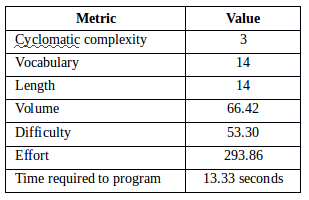
\includegraphics[width=8cm]{figs/cc-values-program-1.png}    
    		\caption{Software metrics for the previous program}
	\end{figure}
\end{center}

\end{frame}

\usebackgroundtemplate{}

%--------------------------------------------------------
\usebackgroundtemplate{
\includegraphics[width=14cm]{figs/goals.jpg}}
%https://rebel-performance.com/wp-content/uploads/2014/10/goals.jpg

\begin{frame}
\frametitle{Research question}

\begin{center}
{\Huge Is the Computational Thinking score given by Dr. Scratch a complexity value that could be compared with the classic software engineering metrics? }
\end{center}
\vspace{2cm}
\hfill{\Tiny Background picture: rebel-performance.com}
\end{frame}

\usebackgroundtemplate{}

%--------------------------------------------------------
\begin{frame}
\frametitle{Methodology}

\begin{itemize}
  \item Random selection of 25 projects of each of the following categories:
  \begin{enumerate}
    \item stories
    \item animations
    \item games
    \item and art creations.
   \end{enumerate} 
   \item Although 100 projects were downloaded, 5 of them produced an error while being analyzed, which limits the sample size to 95 projects.
   \item We developed a plug-in to obtain CC and Halstead from Scratch projects
   \item The mean score was 13.75, while both median and mode were 15. 
\end{itemize}
\end{frame}


%-----------------------    ---------------------------------

\begin{frame}
\frametitle{Correlation between Dr. Scratch and CC and Halstead}
\begin{center}
	\begin{figure}[t!]
		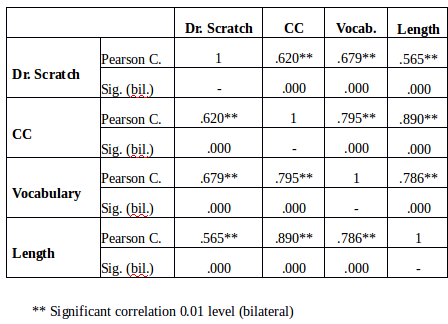
\includegraphics[width=9cm]{figs/correlation.png}    
    		\caption{Correlation between Dr. Scratch and CC and Halstead}
	\end{figure}
\end{center}

\end{frame}

\usebackgroundtemplate{}

%-----------------------    ---------------------------------

\begin{frame}
\frametitle{Correlation by dimension}
\begin{center}
	\begin{figure}[t!]
		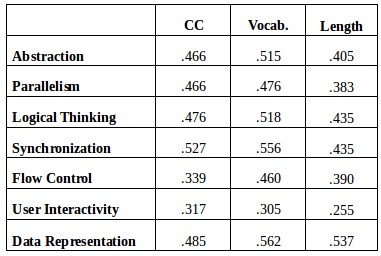
\includegraphics[width=9cm]{figs/correlation-dimensions.png}    
    		\caption{Correlation by dimension}
	\end{figure}
\end{center}

\end{frame}

\usebackgroundtemplate{}

%%--------------------------------------------------------
\usebackgroundtemplate{
\includegraphics[width=13cm]{figs/take-away.jpg}}
%% background: http://flamingcow.co.uk/wp-content/uploads/2015/02/takeaway-940x283.jpg

\begin{frame}
\frametitle{In short...}

  \begin{itemize}
    \item There is correlation between Dr. Scratch CT score and McCabe's Cyclomatic Complexity and Halstead's metrics
    \item Provides validation of the complexity assessment process of Dr. Scratch
    \begin{itemize}
      \item The range of Dr. Scratch CT scores, from 0 to 21 points, could not be flexible enough to represent the differences of complexity for complex projects
      \item An increment in the range of the evaluation of dimensions could enhance correlation
    \end{itemize}
    \item But beware... not everything is (computational) complexity!
  \end{itemize}

\hfill{\Tiny Background picture: flamingcow.co.uk}
%
\end{frame}

\usebackgroundtemplate{}

%--------------------------------------------------------
\frame{
\maketitle
\begin{center}

\includegraphics[width=2cm]{format/libresoft-logo}
\hspace{0.5cm}

\includegraphics[width=5cm]{format/gsyc-urjc}
\vspace{0.5cm}

\includegraphics[width=3cm]{format/emadrid.png}
\end{center}
}

\end{document}
